% Created 2024-10-16 śro 21:35
% Intended LaTeX compiler: pdflatex
\documentclass[../main.tex]{subfiles}

% \usepackage[a4paper, margin=3cm]{geometry}
% \usepackage{amssymb} // not working

\usepackage[T1]{fontenc}
\usepackage[utf8]{inputenc}
\usepackage{graphicx}
\usepackage{longtable}
\usepackage{wrapfig}
\usepackage{rotating}
\usepackage[normalem]{ulem}
\usepackage{amsmath}
\usepackage{capt-of}
\usepackage{hyperref}
\usepackage{siunitx}
\usepackage{float}
\usepackage[polish]{babel}

\graphicspath{{../}}
\author{Wojciech Paderewski}
\date{\today}
\title{Schemat projektu}
\hypersetup{
 pdfauthor={Wojciech Paderewski},
 pdftitle={Schemat projektu},
 pdfkeywords={},
 pdfsubject={},
 pdflang={Polish}}

\begin{document}
Następnym etapem było rozbicie ogólnej koncepcji układu na konkretne rozwiązania projektowe.
Korzystając z wiedzy z rozdziałów \ref{sec:nixie} i \ref{sec:esp32} oraz po zapoznaniu się z ofertą sklepów elektronicznych,
zdecydowano się na poszczególne rozwiązania projektowe, które zostały opisane w dalszej części tego rozdziału.

\subsubsection{Sterowanie lampi nixie}
Kluczowym jest wybór sterownia lampami nixie, ponieważ na podstawie tego wyboru zostanie zaprojektowany reszta układu.
Zgodnie z analizą przeprowadzoną w podrozdziale \ref{sec:sterownie_lampi}, zdecydowano się na sterowanie lampami za pomocą rejestrów przesuwnych HV.
Zastosowanie tego rozwiązania pozwala na zredukowanie ilości potrzebnych pinów mikrokontrolera do sterowania lampami oraz jest to rozwiązanie proste w implementacji.

Niezależnie od wyboru lamp każda ma 10 katod z cyframi i jedną katode od kropki dziesiętnej, więc potrzebujemy 11 wyjść na każdą lampę.
Dostępne w sprzedaży są rejestry 32 bitowe, co pozwala na sterowanie 3 lampami nixie bez kropek i jedną neonówką która bedzie
służyć jako separator między godzinami a minutami oraz między minutami a sekundami. Do sterownia kropkami dziesiętnymi zostaną użyte tranzystory HV podpięte do wyjść mikrokontrolera,
ponieważ nie opłacalnym jest dodawanie kolejnego rejestru przesuwnego HV tylko do sterowania kropkami dziesiętnymi.

Wynika z tego, że potrzebne są 2 rejestry przesuwne HV do sterownia lampi i neonówkami oraz 6 transystorów HV do sterowania kropkami dziesiętnymi.
Do sterowania rejestrami prawdopodobnie będzie potrzebny konwerter poziomów logicznych, ponieważ mikrokontroler ESP32-S3 pracuje na 3.3V, a rejestry prawdopodobnie będą operować na wyższym napięciu.
\subsubsection{Mikrokontroler}
Wybór sposobu sterowania lampami nixie wpłynął na wybór mikrokontrolera, ponieważ musi on posiadać odpowiednią ilość pinów GPIO oraz musi być w stanie generować sygnał zegarowy.
Potrzebne jest 9 pinów GPIO do pełengo sterownia lampami oraz kropkami dziesiętnym, do tego trezba pamiętać o zapasie pinów na pozostałe funkcje. W zwiazku z tym
wybrano mikrokontroler ESP32-S3, który posiada 45 programowalnych GPIO, co pozwala na swobodne zaprojektowanie reszty układu. Ma też on dużą zaletę w postaci kontrolera USB/JTAG,
dzięki czemu nie potrzebujemy dodatkowego programatora do programowania układu. Jest to też popularny mikrokontroler dla którego istnieje dużo bibliotek i przykładów.

\subsubsection{Źródło dźwięku}
Jako źródło dźwięku wybrano głośnik piezoelektryczny, który jest prosty w implementacji i nie wymaga dodatkowego wzmacniacza, do tego jest mały i tani.
Wystarczy jedynie podłączyć go do pinu GPIO mikrokontrolera i za pomocą PWM można generować proste melodie. Głośnik piezoelektryczny jest wystarczająco głośny
aby być słyszalnym w pomieszczeniu, w którym będzie znajdował się budzik.

\subsubsection{Pasek LED}
Pasek LED będzie służył jako dodatkowe źródło światła, które będzie sygnalizować alarm i jako element estetyczny. Pasek ten musi 
zawierać w sobie adresowane diody LED, które pozwolą na wyświetlanie różnych kolorów(RGB).
Rozwiązanie to jest proste w implementacji, wystarczy podłączyć go do pinu GPIO mikrokontrolera i za pomocą PWM można sterować jasnością.

\subsubsection{Interfejs użytkownika}
Interfejs użytkownika będzie składał się z enkodera z przyciskiem, który będzie służył do regulacji jasności, a przycisk do wyłączania alarmu.
Enkoder jest też na tyle uniwersalny, że można na nim dowolne funkcje ustawień manualnych, ale wygodniejsze jest korzystanie z aplikacji mobilnej.

\subsubsection{Zasilanie}
Kluczowe jest zaprojektowanie przetwornicy wysokiego napięcia do zasilania lamp nixie, ponieważ jest to najbardziej wymagający element układu.

Możliwe są dwa rozwiązania:
\begin{itemize}
    \item Przetwornica typu flyback
    \item Przetwornica typu boost
\end{itemize}

Przetwornica typu flyback ma zaletę w postaci izolacji galwanicznej między wejściem a wyjściem oraz jest możliwe zaprojektowanie przetwornicy z napięciem zasilanie 5V
co by pozwoliło na użycie zasilacza USB. Wadą jest to, że jest potrzebny transformator który jest drogi i trudno dostępny, do tego jest to bardziej skomplikowane rozwiązanie na 
etapie projektowania.

Ze względu na duży problem ze znalezieniem transformatora, zdecydowano się na przetwornicę typu boost, która jest prostsza w implementacji i tańsza. Natomiast wymagało
to zastosowania zasilania 12V, co uniemożliwia użycie tylko złącza USB do zasilania układu, natomiast znacząco upraszcza projektowanie układu.

Wybrano więc przetwornicę typu boost, która będzie zasilana z zasilacza 12V, a wyjście będzie podłączone do anod lamp nixie.

Do tego będzie potrzebne zasilanie 5V dla paska LED oraz 3.3V dla mikrokontrolera. Zasilanie 5V w związku z tym, że będzie zasilał pasek LED, który potrafi pobrać większy prąd,
to ze względu na zachowanie wysokiej efektywności, zdecydowano się na przetwornicę typu buck. Zasilanie 3.3V będzie zasilaniem mikrokontrolera, więc wystarczy zastosować
stabilizator liniowy.

Można, więc podzielić zasilanie na 3 pod moduły:
\begin{itemize}
    \item Przetwornica typu boost z zasilacza 12V na HV
    \item Przetwornica typu buck z zasilacza 12V na 5V
    \item Stabilizator liniowy z zasilacza 5V na 3.3V
\end{itemize}

\subsubsection{Złącza}
W związku z tym, że będzie potrzebne zasilanie z zasilacza 12V, zdecydowano się na zastosowanie złącza DC jack, które jest powszechnie stosowane w zasilaczach.
Do zasilania mikrokontrolera oraz programowania, zdecydowano się na złącze USB-C, które jest ocenie najbardziej uniwersalnym rozwiązaniem.
Zostanie również dodane złącze Goldpin, które będzie służyło jako złącze debugowe, co pozwoli na łatwe debugowanie układu, na etapie tworzenia oprogramowania.

Urządzenie będzie posiadać 3 złącza:
\begin{itemize}
    \item Złącze USB-C do programowania mikrokontrolera
    \item Złącze DC do zasilania układu
    \item Złącze Goldpin jako złącze debugowe
\end{itemize}

\subsubsection{Obudowa}
By zachować wygląd retro, zdecydowano się na zastosowanie obudowy drewnianej. Od góry będzie znajdowało się szkło akrylowe, które będzie służyło jako osłona przed kurzem
i jednocześnie będą widoczne elementy elektryczne.

\subsubsection{Szczegółowy schemat projektu}
\begin{figure}[H]
    \centering
    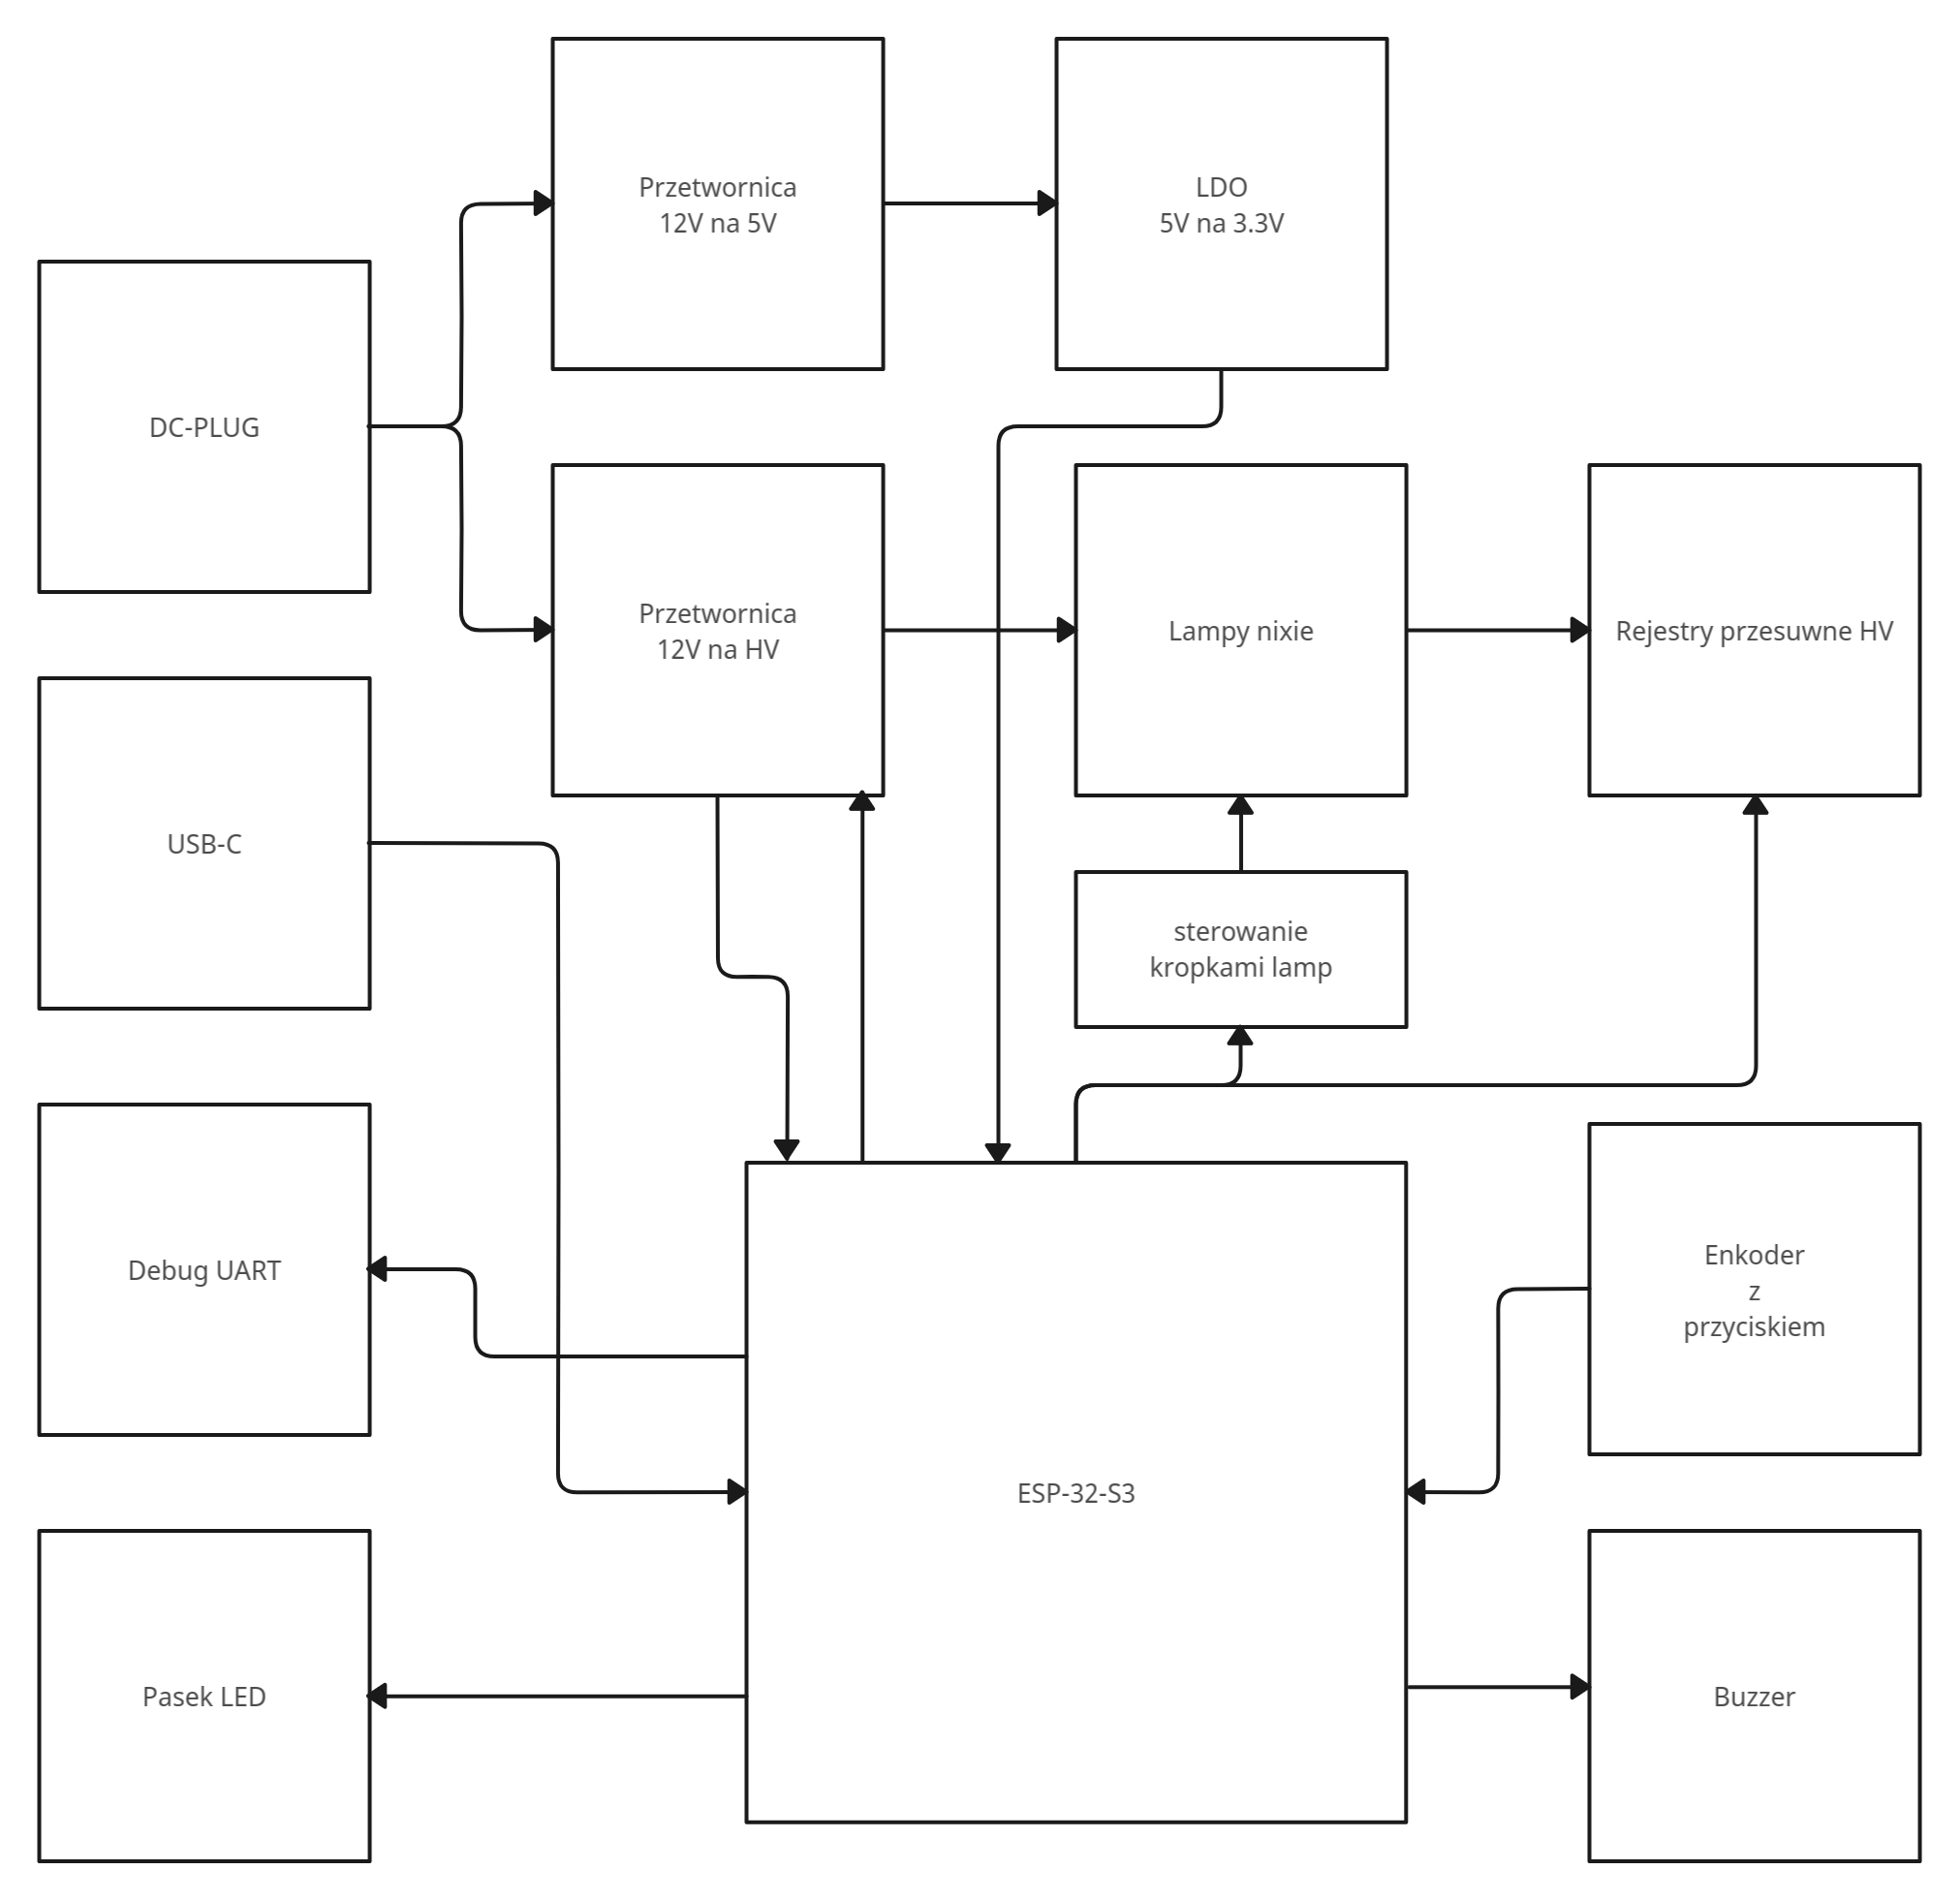
\includegraphics[width=1\textwidth]{schemat_blokowy.jpg}
    \caption{Schemat blokowy projektu}
    \label{fig:schemat_projektu}
\end{figure}

\end{document}
